\section{函数线性无关性}\label{sec:12}

设 $A_i(x) \in \mathbf{Q}[\! [x]\!]$ 为某有限集 $S$ 上的 $\mathbf{P}^1 \setminus S$ 上的全纯函数族（在我们的情况下，它们都将是 Siegel G-函数）。假设我们希望证明 $A_i(x)$ 在 $\mathbf{Q}(x)$ 或 $\mathbf{C}(x)$ 上是线性无关的。一种策略如下：设 $\gamma$ 为 $\mathbf{C}$ 中的一条路径，例如一条从 $x = 0$ 出发，避开 $S$ 中的其他点，然后返回到 $0$ 的路径。函数 $A_i(x)$ 可以沿着 $\gamma$ 解析延拓，而在我们返回 $x = 0$ 时，我们得到一组函数 $\widehat{A}_i(x)$，它们现在可能在 $x = 0$ 处具有奇点。当然，$A_i(x)$ 之间的任何多项式关系都可以延拓为 $\widehat{A}_i(x)$ 之间（相同的）多项式关系，从而也延拓为 $\widehat{A}_i(x) - A_i(x)$ 之间的多项式关系，这有时非常有用。但我们也可以考虑 $\widehat{A}_i(x)$ 在模在 $0$ 处全纯的函数意义下的任何恒等式。原则上可能（且经常）发生的是，这将许多函数之间的线性关系简化为更少函数之间的线性关系，从而人们可以期望采用某种归纳策略来建立完整的线性无关性。一个典型的例子如下：假设路径 $\gamma$ 从 $0 \in S$ 出发，是围绕单点 $1 \in S$ 的简单回路。那么，如果函数 $A_i(x)$ 的一个真子集在 $x = 1$ 处实际上是全纯的，则相应的 $\widehat{A}_i(x)$ 在模全纯函数时消逝，我们便得到了具有更少项的关于 $\widehat{A}_i(x)$ 的相应线性关系。这方面的一个基本例子如下：假设
\[ A_1(x) = 1, \quad A_2(x) = \log(1 - x), \quad A_3(x) = \operatorname{Li}_2(x). \]
在绕 $0$ 旋转一周的合适朝向的回路后，我们有：
\[ \widehat{A}_1(x) = 1, \quad \widehat{A}_2(x) = \log(1 - x) + 2\pi i, \quad \widehat{A}_3(x) = \operatorname{Li}_2(x) + 2\pi i \log(x). \]
现在，在模 $0$ 处全纯的函数时，我们得到这三个函数 $0$、$0$ 和 $2\pi i \log(x)$ 之间的一个线性关系。显然，这迫使 $\widehat{A}_3(x)$ 的系数为零，并将我们简化为说明 $A_1(x)$ 和 $A_2(x)$ 线性无关，因为 $\log(1-x)$ 不是有理函数。我们将在下文多次使用该策略。请注意，在此情形下的另一种论证是考虑函数 $\widehat{A}_i(x) - A_i(x)$，这能将问题简化为 $1$ 与 $\log x$ 的 $\mathbf{C}(x)$-线性无关性。

\begin{mylemma}{}{lem:12.0.1}
在第 10 节中分别由方程 \eqref{eq:10.1.2}、\eqref{eq:10.1.3} 和 \eqref{eq:10.2.1} 定义的七个函数 $B_i(y)$（$i = 1, \dots, 7$）在 $\mathbf{C}(y)$ 上是线性无关的。
\end{mylemma}

\begin{proof}
我们首先注意到 $B_i(y)$ 均是 $\mathbf{Q}[\! [y]\!]$ 的元素。因此，任何在 $\mathbf{C}(y)$ 上的线性相关性都可以提升到 $\mathbf{Q}(y)$ 上，因而只需在 $\mathbf{Q}(y)$ 上证明该结果即可。

我们首先证明 $B_i(y)$（对 $i = 1, \dots, 5$）的线性无关性。根据\mylem{lem:9.0.3}，只需在 $\mathbf{Q}(x)$ 上证明 5 个函数 $1$、$\log(1-x)$、$\log^2(1-x)$、$\operatorname{Li}_2(x)$ 以及式 \eqref{eq:10.1.5} 中的 $J(x)$ 的线性无关性。显然，$1$、$\log(1-x)$ 和 $\log^2(1-x)$ 线性无关，因为 $\log(1-x)$ 在 $\mathbf{Q}(x)$ 上是超越的。这三个函数也定义在 $\mathbf{P}^1 \setminus \{1,\infty\}$ 上，这使它们与 $\operatorname{Li}_2(x)$ 区分开来——考虑一条从 0 出发的路径 $\gamma$，该路径绕 $x=1$ 旋转，然后绕 $x=0$ 旋转，接着以相反的方向绕 $x=1$ 旋转，最后返回到零（如图 \ref{fig:12.0.7} 所示）。前三个函数在这一路径上是保持不变的，但 $\operatorname{Li}_2(x)$ 在该路径上具有非平凡的单值性（monodromy）。因此，$\operatorname{Li}_2(x)$ 独立于这些先前的函数。现在，假设 $J(x)$ 是 $1, \log(1-x), \log^2(1-x), \operatorname{Li}_2(x)$ 的 $\mathbf{Q}(x)$-线性组合。如果 $\operatorname{Li}_2(x)$ 的系数是非平凡的，那么在缩放后，我们可以假设它是 1。但现在通过求导并利用关于 $J(x)$ 的常微分方程 \eqref{eq:10.1.6}，我们获得了一个仅有 $1, \log(1-x), \log^2(1-x)$ 和 $J(x)$ 的在 $\mathbf{Q}(x)$ 上的新关系（由于常微分方程， $J(x)$ 具有非平凡系数）。但是 $J(x)$ 沿着路径 $\gamma$ 也具有非平凡的单值性，因此我们同上文的 $\operatorname{Li}_2(x)$ 一样得出相同的结论。

现在让我们回到 $\mathbf{P}^1 \setminus \{0,4,\infty\}$ 区域，并考虑函数 $B_6(y)$ 和 $B_7(y)$。回忆：
\[ B_6(y) = \int \frac{B_3(y)}{y} \, dy, \quad B_7(y) = \int \frac{B_4(y)}{y} \, dy. \]
利用求导公式：
\begin{equation}\label{eq:12.0.2}\tag{12.0.2}
\frac{d}{dy} \left\{ A(y) \int F(y) \, dy \right\} = A'(y) \int F(y) \, dy + A(y) F(y),
\end{equation}
我们首先可以假设 $\mathbf{Q}(y)$ 中的线性关系的系数是多项式，然后通过求导将其化简为具有如下形式的等式：
\begin{equation}\label{eq:12.0.3}\tag{12.0.3}
a_0 \int \frac{B_3(y)}{y} dy + a_1 \int \frac{B_4(y)}{y} dy = \sum_{i=1}^5 b_i(y) B_i(y),
\end{equation}
其中 $a_0$ 和 $a_1$ 是不全为零的常数，且 $b_i(y) \in \mathbf{Q}(y)$。

我们注意到：
\begin{equation}\label{eq:12.0.4}\tag{12.0.4}
\begin{aligned}
y(4-y)\frac{d}{dy}B_{2}(y) &= (2-y)B_{2}(y) + y^{2}, \\
y(4-y)\frac{d}{dy}B_{3}(y) &= -B_{2}(y) + 2y, \\
y(4-y)\frac{d}{dy}B_{4}(y) &= (2-y)B_{4}(y) + (4-y)B_{2}(y) - 2y(4-y), \\
2y(4-y)\frac{d}{dy}B_{5}(y) &= (4-y)B_{5}(y) - 2B_{2}(y) + 4y.
\end{aligned}
\end{equation}

但现在，让我们对 \eqref{eq:12.0.3} 进行求导以得到：
\begin{equation}\label{eq:12.0.5}\tag{12.0.5}
a_0 \frac{B_3(y)}{y} + a_1 \frac{B_4(y)}{y} = \sum_{i=1}^5 \left( b_i(y) B_i'(y) + b_i'(y) B_i(y) \right).
\end{equation}
我们从方程 \eqref{eq:12.0.4} 并且通过分别比较 $B_4(y)$ 和 $B_3(y)$ 的系数（并利用 $B_i(y)$ 对 $i = 1, \dots, 5$ 的线性无关性）可以看出：
\begin{equation}\label{eq:12.0.6}\tag{12.0.6}
\frac{a_0}{y} = b_3'(y), \qquad \frac{a_1}{y} = b_4'(y) + \frac{(2-y)}{y(4-y)}b_4(y).
\end{equation}
从前一个方程，我们得到（在相差常数意义下）：
\[ b_3(y) = a_0 \log(y), \]
因为 $b_3(y) \in \mathbf{Q}(y)$，这只有在 $a_0 = 0$ 时才会发生。我们也可以将第二个方程写为：
\[ \frac{a_1\sqrt{y(4-y)}}{y} = \frac{d}{dy}\left(b_4(y)\sqrt{y(4-y)}\right). \]
但是左半部分的积分（若 $a_1 \neq 0$）是非代数的，而右半部分的积分是代数的，所以这再次只能在 $a_1 = 0$ 时发生，由此建立了线性无关性。


\end{proof}


\begin{figure}[htbp]
\centering
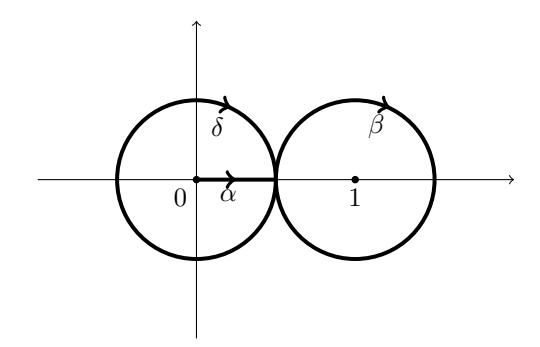
\includegraphics[width=0.6\textwidth]{assets/fig/_page_166_Figure_2.jpeg}
\caption{路径 $\gamma = \alpha^{-1}\beta^{-1}\delta\beta\alpha$.}\label{fig:12.0.7}
\end{figure}

\subsection{纯函数与 Zagier 函数的线性无关性}\label{sec:12.1}

回忆由\rdef{def:11.2.1}：
\[ G(y) = H(x) + H\left(\frac{x}{x-1}\right). \]
我们还设：
\[ G_A(y) = H_A(x) + H_A\left(\frac{x}{x-1}\right) \in \mathbf{Z}[\! [y]\!], \]
它是下面方程 \eqref{eq:12.1.5} 中显式给出的一个 4 阶齐次常微分方程的解。我们最后的函数线性无关性结果如下：

\begin{mylemma}{14 个函数}{lem:12.1.1}
七个函数
\[ \int G(y) dy, \quad \int \frac{G(y) - G(0)}{y} dy, \quad \int \frac{G(y) - G(0) - G'(0)y}{y^2} dy, \]
\[ G(y), \quad G'(y), \quad G''(y), \quad G'''(y), \]
以及这七个函数 $B_i(y)$（对 $i = 1, \dots, 7$），在 $\mathbf{C}(y)$ 上是线性无关的。
\end{mylemma}

\begin{remark}\label{rem:12.1.2}
通过实验来发现\mylem{lem:12.1.1}是相当容易的。一族在 $\mathbf{C}(y)$ 上满足线性关系的幂级数 $A_i(x)$，也在 $\mathbf{C}[y]$ 中满足一个线性关系，因此其系数为次数不超过 $D$ 的多项式（对于某个 $D \in \mathbf{N}_{>0}$）。但是，对于任何给定的 $D$ 是否存在这样的关系，等价于一个显式可计算矩阵的行列式是否消逝。一旦确立了对于中等大小的 $D$（例如 $D = 20$）不存在这样的线性关系，人们就会充分相信该结果是正确的，然后写下证明。我们承认，这正是我们得出\mylem{lem:12.1.1}和引理~14.3.1 的方式，尽管极有可能存在一个能更好地解释这套精密数字的高观点证明。参见\rremark{rem:12.1.12}。\end{remark}

\begin{proof}
由于根据\mylem{lem:12.0.1}，$B_i(y)$ 是线性无关的，任何线性相关关系必定包含至少一个上述带有非零系数的 $G$ 的项。设 $\gamma$ 表示如下路径：首先穿过 $4$，然后穿过 $-1/72$，接着以相反的方向穿过 $4$，最后回到 $0$。函数 $G(y)$ 被替换为 $\widehat{G}(y)$，它是满足与 $G(y)$ 相同的非齐次微分方程的解。另一方面，函数 $\widehat{B}_n(y) = B_n(y)$ 保持不变。由于 $G(y) \neq \widehat{G}(y)$， we 得到了具有相同系数的函数：
\[ \int \widehat{G}(y) \, dy, \quad \int \frac{\widehat{G}(y) - G(0)}{y} \, dy, \quad \int \frac{\widehat{G}(y) - G(0) - G'(0)y}{y^2} \, dy, \]
\[ \widehat{G}(y), \quad \widehat{G}'(y), \quad \widehat{G}''(y), \quad \widehat{G}'''(y) \]
与 $B_i(y)$ 之间的等价线性关系。因此，设 $\Delta = \widehat{G}(y) - G(y)$，我们得到了以下七个函数之间的非零 $\mathbf{C}(y)$-线性关系：
\[ \int \Delta(y) \, dy, \quad \int \frac{\Delta(y)}{y} \, dy, \quad \int \frac{\Delta(y)}{y^2} \, dy, \quad \Delta(y), \quad \Delta'(y), \quad \Delta''(y), \quad \Delta'''(y). \]
但是，$\Delta(y)$ 现在是对应的 4 阶不可约齐次常微分方程（ODE）的解。因此，通过用 $\Delta(y)$ 在单值群 $\pi_1(\mathbf{P}^1 \setminus \{0, -1/72, 4, \infty\})$ 的元素作用下的变换来替换它，我们推导出相应的线性关系必须对任何这样的 $\Delta(y)$ 均成立，特别地，包括全纯解 $\Delta(y) = G_A(y)$。

假设存在这样一个线性关系。在缩放之后，我们可以假设系数位于 $\mathbf{C}(y)$ 中。再次使用求导公式：
\begin{equation}\label{eq:12.1.3}\tag{12.1.3}
\frac{d}{dy} \left\{ A(y) \int F(y) \, dy \right\} = A'(y) \int F(y) \, dy + A(y)F(y).
\end{equation}
在反复求导之后，我们可以假设三个积分项的系数都是常数，并且至少有一个是非零的。因此存在关系：
\begin{equation}\label{eq:12.1.4}\tag{12.1.4}
a_0 \int G_A(y) \, dy + a_{-1} \int \frac{G_A(y)}{y} \, dy + a_{-2} \int \frac{G_A(y)}{y^2} \, dy = \sum_{i=0}^3 b_i(y) G_A^{(i)}(y).
\end{equation}
请注意，我们不能坚持要求 $b_i(y) \in \mathbf{C}[y]$，原因有两个。第一，来自积分的导数项涉及 $G_A(y)$ 除以 $y$ 的幂次。第二，在对 $G_A^{(3)}(y)$ 进行求导时，我们得到了 $G_A^{(4)}(y)$，要将其用较低阶导数 $G_A^{(i)}(y)$ 表达，我们需要除以微分方程中的领先项（leading term）。

实际上，$G_A(y)$ 满足如下常微分方程（ODE）：
\[ \sum_{i=0}^{4} c_i(y) G_A^{(i)}(y) = 0, \]
其中 $c_i(y)$ 定义如下：
\begin{equation}\label{eq:12.1.5}\tag{12.1.5}
\begin{aligned}
c_{0}(y) &= -18(3 + 126y - 712y^{2} + 360y^{3}), \\
c_{1}(y) &= 2(-2 - 2761y + 141632y^{2} - 280328y^{3} + 176412y^{4} - 95616y^{5} + 20736y^{6}), \\
c_{2}(y) &= 2y(-34 - 6353y + 690355y^{2} - 1065613y^{3} + 867876y^{4} - 438336y^{5} + 72576y^{6}), \\
c_{3}(y) &= 2(-4 + y)y^{2}(10 + 204y - 118195y^{2} + 146946y^{3} - 142848y^{4} + 41472y^{5}), \\
c_{4}(y) &= (-4 + y)^{2}y^{3}(1 + 72y)(-1 + 118y - 122y^{2} + 144y^{3}).
\end{aligned}
\end{equation}

因此我们可以假设 $b_i(y) \in \mathbf{C}[y, c_4(y)^{-1}]$。将方程 \eqref{eq:12.1.4} 再进行一次求导，可以得到恒等式：
\begin{equation}\label{eq:12.1.6}\tag{12.1.6}
a_0 G_A(y) + a_{-1} \frac{G_A(y)}{y} + a_{-2} \frac{G_A(y)}{y^2} = \sum_{i=0}^3 \left( b_i'(y) G_A^{(i)}(y) + b_i(y) G_A^{(i+1)}(y) \right).
\end{equation}
我们将 \eqref{eq:12.1.6} 重写为：
\begin{equation}\label{eq:12.1.7}\tag{12.1.7}
\begin{aligned}
a_0 G_{A}(y) + a_{-1} \frac{G_{A}(y)}{y} + a_{-2} \frac{G_{A}(y)}{y^{2}} &= \sum_{i=0}^{3} b'_{i}(y)G_{A}^{(i)}(y) + \sum_{i=1}^{3} b_{i-1}(y)G_{A}^{(i)}(y) + b_{3}(y)G_{A}^{(4)}(y) \\
&= \sum_{i=0}^{3} b'_{i}(y)G_{A}^{(i)}(y) + \sum_{i=1}^{3} b_{i-1}(y)G_{A}^{(i)}(y) - \sum_{i=0}^{3} \frac{c_{i}(y)}{c_{4}(y)}b_{3}(y)G^{(i)}(y),
\end{aligned}
\end{equation}
由此我们推导出联立方程组：
\begin{equation}\label{eq:12.1.8}\tag{12.1.8}
\begin{aligned}
b'_{3}(y) + b_{2}(y) - \frac{c_{3}(y)}{c_{4}(y)}b_{3}(y) &= 0, \\
b'_{2}(y) + b_{1}(y) - \frac{c_{2}(y)}{c_{4}(y)}b_{3}(y) &= 0, \\
b'_{1}(y) + b_{0}(y) - \frac{c_{1}(y)}{c_{4}(y)}b_{3}(y) &= 0, \\
b'_{0}(y) - \frac{c_{0}(y)}{c_{4}(y)}b_{3}(y) &= a_{0} + \frac{a_{-1}}{y} + \frac{a_{-2}}{y^{2}}.
\end{aligned}
\end{equation}

回忆 $b_3(y) \in \mathbf{C}[y, c_4(y)^{-1}]$。此外，给定 $b_3(y)$，人们可以从以下方程归纳地解出 $b_i$（其中 $i \in \{2, 1, 0\}$）：
\[ b_i(y) = \frac{c_{i+1}(y)}{c_4(y)}b_3(y) - b'_{i+1}(y). \]
我们的策略如下：由于 $b_3(y) \in \mathbf{C}(y)$，我们可以考虑 $b_3(y)$ 围绕 $\infty$ 级任意复数点 $\alpha \in \mathbf{C}$ 的幂级数展开。然后，通过考虑最后的等式，我们获得了关于 $b_3(y)$ 在 $\alpha$ 处任意极点阶数的显式边界（请注意，除非 $\alpha = \infty$ 或是 $c_4(y)$ 的根，否则 $b_3(y)$ 将是全纯的）。但这将 $b_3(y)$ 限制为一个有理函数，使得因子 $\operatorname{divisor}(b_3(y)) + D \ge 0$（其中显式除子 $D$ 支撑在 $c_4(y)$ 的根处）。这是一个有限维的（显式可计算的）向量空间，然后我们可以使用线性代数来求解所有可能的 $b_3(y)$。另一种看待这一点的方式是将该系统视为 $b_3(y)$ 的（非齐次）常微分方程，并且我们正在使用 Frobenius 方法计算围绕任意点的（可能）局部展开。显式地，设 $\alpha \neq \infty$，并且
\[ b_3(y) = \sum_{i=N}^{\infty} r_i (y - \alpha)^i, \]
（其中 $N = N_{\alpha}$，$r_i = r_{i,\alpha}$，我们在下面省略了下标），则：
\begin{enumerate}
\item[(1)] 若 $\alpha = 0$，最后的等式变为：
\[ a_0 + \frac{a_{-1}}{y} + \frac{a_{-2}}{y^2} = \frac{-1}{4}(3-N)^2(5-2N)^2r_Ny^{N-4} + \dots \]
\item[(2)] 若 $\alpha = 4$，最后的等式变为：
\[ a_0 + \frac{a_{-1}}{y} + \frac{a_{-2}}{y^2} = \frac{-1}{4}(3-N)(2-N)(5-2N)(3-2N)r_N(y-4)^{N-4} + \dots \]
\item[(3)] 若 $\alpha = -1/72$，最后的等式变为：
\[ a_0 + \frac{a_{-1}}{y} + \frac{a_{-2}}{y^2} = (3 - N)^2 (2 - N)(1 - N)r_N (y + 1/72)^{N-4} + \dots \]
\item[(4)] 若 $\alpha$ 是 $144y^3 - 122y^2 + 118y - 1 = 0$ 的根 $\beta$，则：
\[ a_0 + \frac{a_{-1}}{y} + \frac{a_{-2}}{y^2} = (3 - N)(2 - N)(1 - N)(1 + N)r_N(y - \beta)^{N-4} + \dots \]
\item[(5)] 在 $\alpha \to \infty$ 处，设：
\[ b_3(y) = y^N \sum_{i=N}^{\infty} r_i y^{-i}, \]
我们有：
\[ a_0 + \frac{a_{-1}}{y} + \frac{a_{-2}}{y^2} = \frac{-1}{4}(3-N)^2(5-2N)^2r_Ny^{N-4} + \dots \]
\end{enumerate}

由此我们推导出：
\begin{equation}\label{eq:12.1.9}\tag{12.1.9}
N_{0} \ge 2, \qquad N_{4} \ge 2, \qquad N_{-1/72} \ge 1, \qquad N_{\beta} \ge -1, \qquad N_{\infty} \le 4.
\end{equation}
由此可得：
\begin{equation}\label{eq:12.1.10}\tag{12.1.10}
b_3(y) = \frac{y^2(y-4)^2(y+1/72)}{(144y^3 - 122y^2 + 118y - 1)}Q(y),
\end{equation}
其中 $Q(y)$ 为次数至多为 2 的多项式。然而，如果我们写成：
\[ Q(y) = q_0 + q_1 y + q_2 y^2, \]
那么我们发现：
\begin{equation}\label{eq:12.1.11}\tag{12.1.11}
a_0 + \frac{a_{-1}}{y} + \frac{a_{-2}}{y^2} = \frac{52542464y^{12}q_2 + \dots}{36y^2(-1 + 118y - 122y^2 + 144y^3)^4},
\end{equation}
其中右边的分子是 12 次多项式，其系数关于 $q_0, q_1, q_2$ 是线性的。但现在通过线性代数，人们可以直接检查发现，根本没有参数 $q_i$ 的选择能使分子在分母的非零根处消逝至（至少）一阶。因此，不存在这样的 $b_3(y)$，证明完毕。
\end{proof}

\begin{remark}\label{rem:12.1.12}
假设相反地，我们曾尝试证明这七个函数 $B_i(y)$ 与如下函数之间的（错误的！）线性无关性：
\[
\begin{aligned}
&\int G(y) dy, \quad \int \frac{G(y)-G(0)}{y}dy, \quad \int \frac{G(y)-G(0)-G'(0)y}{y^{2}}dy, \\
&\quad \int \frac{G(y)-G(0)-G'(0)y-G''(0)y^{2}}{y^{3}}dy,
\end{aligned}
\]
\[ G(y), \quad G'(y), \quad G''(y), \quad G'''(y), \]
也就是说，加入另外一个积分。那么论证将完全同上文进行，除了现在我们只能推导出 $N_0 \ge 1$ 而非 $N_0 \ge 2$。然后，写成：
\[ Q(y) = \frac{q_{-1}}{y} + q_0 + q_1 y + q_2 y^2, \]
就像方程 \eqref{eq:12.1.11} 中那样，我们将发现：
\[ a_0 + \frac{a_{-1}}{y} + \frac{a_{-2}}{y^2} + \frac{a_{-3}}{y^3} = \frac{52542464y^{13}q_2 + \dots}{36y^3(-1 + 118y - 122y^2 + 144y^3)^4}. \]
现在，在相差缩放因子意义下，存在唯一的参数 $q_i$ 选择，允许我们消去分子中的单个因子，即（相差常数倍）：
\[ Q(y) = \frac{1}{y} - 278 - 844y - 4644y^{2}. \]
采用来自方程 \eqref{eq:12.1.10} 的这一 $b_3(y)$ 选择，$(144y^3 - 122y^2 + 118y - 1)$ 的幂次完全消失，并且我们到达等式：
\[ a_0 + \frac{a_{-1}}{y} + \frac{a_{-2}}{y^2} + \frac{a_{-3}}{y^3} = \frac{676}{9y^2} + \frac{2}{y^3}. \]
这当然现在有解。这反映了在这些函数之间存在一个线性相关性。事实上，在以下函数之间已经存在一个 $\mathbf{C}(y)$-线性相关性：
\[
\begin{aligned}
& \int \frac{G_A(y)}{y^2} \, dy, \quad \int \frac{G_A(y)}{y^3} \, dy, \quad G_A(y), \\
& \quad G_A'(y), \quad G_A''(y), \quad G_A'''(y) \quad \text{和} \quad 1.
\end{aligned}
\]
作为与解 $a_{-2} = 676/9$ 和 $a_{-3} = 2$ 的另一个相容性检查，我们有（与方程 \eqref{eq:12.1.6} 类比）：
\[ a_0 G_A(y) + a_{-1} \frac{G_A(y)}{y} + a_{-2} \frac{G_A(y)}{y^2} + a_{-3} \frac{G_A(y)}{y^3} = \frac{676}{9} \frac{G_A(y)}{y^2} + 2 \frac{G_A(y)}{y^3} \]
\[ = \frac{4}{y^3} + \frac{866}{9y^2} - \frac{68728}{3} + \dots \]
它不含 $1/y$ 项，这与它是 $y = 0$ 处亚纯函数的导数是一致的。
\end{remark}
